\documentclass[border=0.2cm, convert={density=600}]{standalone}
 
% Required packages and libraries
\usepackage{tikz}
\usetikzlibrary{shapes, positioning, arrows.meta, calc}

% custom styles
\tikzset{
  parser/.style={
    rectangle,
    rounded corners,
    draw=black, very thick,
    minimum height=2em,
    inner sep=2pt,
    text centered,
    rectangle split,
    rectangle split draw splits=false,
    rectangle split parts=2,
    draw=black
  },
  arrow/.style={
    draw=black,
    thick,
    ->,
    >=stealth
  }
}

% custom dot symbol (bigger than \cdot but smaller than \bullet)
\makeatletter
\newcommand*\dotp{\mathpalette\dotp@{.5}}
\newcommand*\dotp@[2]{\mathbin{\vcenter{\hbox{\scalebox{#2}{$\m@th#1\bullet$}}}}}
\makeatother
 
\begin{document}
 
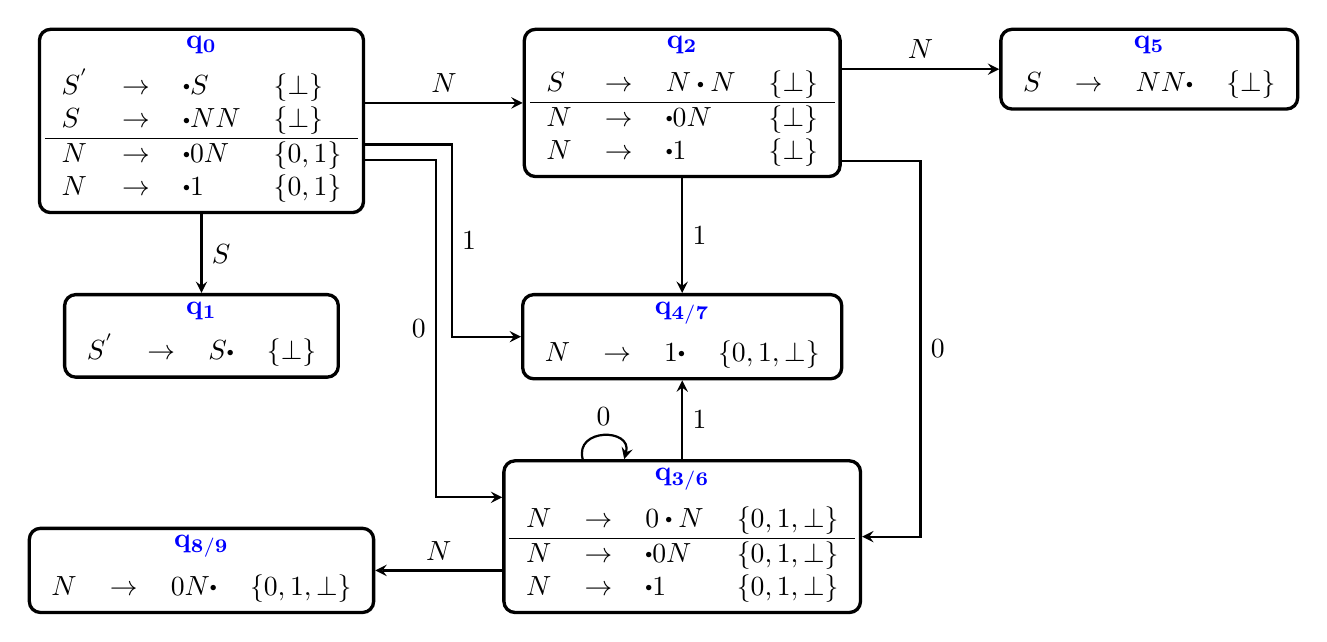
\begin{tikzpicture}
% LR(1) Parser
% Grammar:
%	(0) S' → S
%	(1) S → NN
%	(2) N → 0N
%	(3) N → 1

% nodes
\node[parser] (q0)
{ $\mathbf{\color{blue} q_{0}}$
  \nodepart{second}
  \begin{tabular}{llll}
     $S^{'}$ & $\rightarrow$ & $\dotp S$  & $\lbrace \bot \rbrace$\\
     $S$     & $\rightarrow$ & $\dotp N N$ & $\lbrace \bot \rbrace$\\
     \hline
     $N$     & $\rightarrow$ & $\dotp 0N$ & $\lbrace 0,1 \rbrace$\\
     $N$     & $\rightarrow$ & $\dotp 1$ & $\lbrace 0,1 \rbrace$\\
  \end{tabular}
};

\node[parser, below = 1cm of q0] (q1)
{ $\mathbf{\color{blue} q_{1}}$
  \nodepart{second}
  \begin{tabular}{llll}
     $S^{'}$ & $\rightarrow$ & $S\dotp$ & $\lbrace \bot \rbrace$\\
  \end{tabular}
};

\node[parser, right = 2cm of q0.north east, anchor=north west] (q2)
{ $\mathbf{\color{blue} q_{2}}$
  \nodepart{second}
  \begin{tabular}{llll}
     $S$ & $\rightarrow$ & $N \dotp N$ & $\lbrace \bot \rbrace$\\
     \hline
     $N$ & $\rightarrow$ & $\dotp 0 N$ & $\lbrace \bot \rbrace$\\
     $N$ & $\rightarrow$ & $\dotp 1$   & $\lbrace \bot \rbrace$\\
  \end{tabular}
};

\node[parser, anchor=north] (q47) at (q1.north -| q2.south)
{ $\mathbf{\color{blue} q_{4/7}}$
  \nodepart{second}
  \begin{tabular}{llll}
     $N$ & $\rightarrow$ & $1 \dotp$ & $\lbrace 0,1,\bot \rbrace$\\
  \end{tabular}
};

\node[parser, below = 1cm of q47] (q36)
{ $\mathbf{\color{blue} q_{3/6}}$
  \nodepart{second}
  \begin{tabular}{llll}
     $N$ & $\rightarrow$ & $0 \dotp N$ & $\lbrace 0,1,\bot \rbrace$\\
     \hline
     $N$ & $\rightarrow$ & $\dotp 0 N$ & $\lbrace 0,1,\bot \rbrace$\\
     $N$ & $\rightarrow$ & $\dotp 1$   & $\lbrace 0,1,\bot \rbrace$\\
  \end{tabular}
};

\node[parser, right = 2cm of q2.north east, anchor=north west] (q5)
{ $\mathbf{\color{blue} q_{5}}$
  \nodepart{second}
  \begin{tabular}{llll}
     $S$ & $\rightarrow$ & $N N \dotp$ & $\lbrace \bot \rbrace$\\
  \end{tabular}
};

\node[parser, anchor=south] (q89) at (q36.south -| q1.south)
{ $\mathbf{\color{blue} q_{8/9}}$
  \nodepart{second}
  \begin{tabular}{llll}
     $N$ & $\rightarrow$ & $0 N \dotp$ & $\lbrace 0,1,\bot \rbrace$\\
  \end{tabular}
};

% edges

%% q0
\draw [arrow] (q0.south) -- node[anchor=west]{$S$} (q1.north);
\draw [arrow] (q0.east |- q2.west) -- node[anchor=south]{$N$} (q2.west);

\coordinate[right=0.9cm of q0.east, yshift=-5mm] (h03);
\coordinate[yshift=5mm] (e03) at (q36.west);
\draw [arrow] (q0.east |- h03) -- (h03) -- node[left]{$0$} (h03 |- e03) -- (e03);

\coordinate[right=1.1cm of q0.east, yshift=-3mm] (h04);
\draw [arrow] (q0.east |- h04) -- (h04) -- node[right]{$1$} (h04 |- q47.west) -- (q47.west);


%% q2
\coordinate[right=1cm of q2.-20] (h23) ;
\draw [arrow] (q2.east |- q5.west) -- node[anchor=south]{$N$} (q5.west);
\draw [arrow] (q2.-20) -- (h23) -- node[anchor=west]{$0$} (h23 |- q36.east) -- (q36.east);
\draw [arrow] (q2.south) -- node[anchor=west]{$1$} (q47.north);

%% q36
\draw [arrow] (q36.west |- q89.east) -- node[anchor=south]{$N$} (q89.east);
\path [arrow, every loop/.style={min distance=3mm,looseness=2}] (q36) edge[loop above, transform canvas={xshift=-10mm}] node[anchor=south]{$0$} ();
\path [arrow] (q36.north) -- node[anchor=west]{$1$} (q47.south);
%On d goto (4,7)

\end{tikzpicture}
 
\end{document}
